\newcommand{\Mod}[1]{\text{ (mod } #1\text{)}}
\section{Our Solution and Evaluation}
For the three issues, we will propose available solution in this section.
\subsection{Best GoP}
As mentioned above, the value of GoP needs a tradeoff between video quality and frame dropping. The x264 encoder use the delta intermode coding, thus a larger GoP is much likely to introduce the accumulative errors, and GoP is suggested smaller than 250 frames. But how to determine the value is still an intractable question. To guide the choice of keyframe interval, we try to vary the GoP and encode many original streaming into flv format. The relationship between normalized SSIM and gop size is displayed in Fig. .

From the previous figure, we can see that value between $[20,60]$ is always a better tradeoff.

\subsection{Drop Strategy}

\begin{table}[tb]
\footnotesize
\centering
\caption{Terminology in Integer Program}
\label{tbl:term}
{\setlength{\tabcolsep}{1pt}
\begin{tabular}{|c|c|l|}
\hline
\textbf{Symbol} & \textbf{Type} & \textbf{Meaning}                      \\ \hline
$i$               & index         & frame index                           \\ \hline
$j$               & index         & time index                            \\ \hline
$x_{ij}$             & variable      & whether frame $i$ is in queue at time $j$ \\ \hline
$y_{ij}$             & variable      & whether frame $i$ is sent at time $j$     \\ \hline
$z_{ij}$             & variable      & whether frame $i$ is dropped at time $j$  \\ \hline
$T$               & const         & decision time                        \\ \hline
$T_1$             & const       & max time when a frame keeps ``fresh'' \\ \hline
$C_j$              & const         & network bandwidth at time $j$           \\ \hline
$N$               & const         & key frame interval                      \\ \hline
$S$            & const         & each frame size                        \\ \hline
$M_{j}$       & const         & frame index that can be send at time $j$ \\ \hline
$R_{i}$        & const         & bitrate of the $i$ frame               \\ \hline
\end{tabular}}
\end{table}

\begin{figure}[tb]
\centering
{\setlength{\tabcolsep}{3pt}
\begin{tabular}{|l|l|}
\hline
\multicolumn{2}{|c|}{ maximize $\Sigma_i y_{iT}$, subject to} \\ \hline \hline
 $x_{ij}+y_{ij}+z_{ij} = 0, \forall j<i$       & (1)        \\
 $x_{ij}+y_{ij}+z_{ij} = 1, \forall j\geq i$   & (2)       \\
 $x_{ij} \geq x_{i,j+1}, \forall j\geq i$      & (3)        \\
 $y_{ij} \leq y_{i,j+1}, \forall j\geq i$      & (4)        \\
 $z_{ij} \leq z_{i,j+1}, \forall j\geq i$      & (5)        \\ \hline
 $y_{ij} = \max\{1,{1-z_{i,j-1}}\}, \forall j, i \leq M_{j}$  & (6)   \\ \hline
 $y_{ij}+z_{ij} = 1 ,\forall j>i+T_2$          & (7)        \\ \hline
 $y_{i+1,T} \geq y_{iT}, \forall i \not\equiv N-1 (\text{mod}N)$ &(8) \\ \hline
\end{tabular}}
\caption{Frame Drop Strategy}
\label{fig:ip-program} \mylabel{fig:ip-program}
\end{figure}

\subsubsection{Problem Formulation}
For the constant bitrate case, assume the pace of video frame and network bandwidth are known, there exists an optimal scheduling regarding maximize audience QoE within the system constraints (bandwidth and queue timeliness length). Actually a group of pictures always compose of three kinds of frames, I/P/B frames, here for simpleness, we delete the B frame to solve the fundamental problem. The problem can be formulated by integer programming (Figure~\ref{fig:ip-program}). Terminologies are defined in Table~\ref{tbl:term}. We discretize time into time stamps from $0$ to $T$, and assume the frame with index $i$ is generated at time $i$. We define $x_{ij}$, $y_{ij}$, $z_{ij}$ as 0/1 variables to describe whether a packet is in the queue, sent or dropped.

\textbf{Frame conservation constraints.}
Frame $i$ is generated at time $i$, and after that, it is either in the queue or sent or dropped (1-2).
After a packet is removed from the queue, it would never be enqueued (3).
After a packet is sent/dropped, it is permanently sent/ dropped afterward (4-5).

\textbf{Bandwidth constraints.}
The determination of sending strategy $y_{ij}$, is also an interesting and important problem. However, for simpleness, in this paper we just assume that the streamer sends as many as possible, which is a good choice. This means, at time $j$ we just set all the possible $y_{ij}$ to true. At any time, the number of sent frames does not exceed the network bandwidth. According to these constraints, max frame index $M_{j}$ can be calculated by maximize the function $M_j = argmax(\Sigma_k y_{kj}-y_{k,j-1} \leq C_{j})$. Besides the frame that can be send must be not dropped.

\textbf{Timeliness constraint.}
A frame is ``fresh'' if it is sent with in ``$T_1$''. That is, a frame is either sent or drop after time $T_1$ of its generation (6).

\textbf{Decodability constraints.} The final delivered frames must be decodable; otherwise, they would be a waste of network bandwidth. I frames are always decodable. A P frame is decodable if and only if its preceding I or P frame is decodable(7).

\textbf{Optimization goal.} The goal of the IP model is to maximize the delivered frames.
Compared with prior work~\cite{singh2004dynamic}, this IP model has timeliness and decodability in consideration, thus it is more suitable for personalized live streaming.

 DP can no doubt achieve the offline optimal. But long-term bandwidth cannot be known ahead of time, so DP cannot be applied in practice. A online drop strategy is necessary.

\subsubsection{Greedy Algorithm}
\begin{algorithm}[tb]
\caption{GreedyDrop Algorithm}
\label{alg:greedy-drop}\mylabel{alg:greedy-drop}
\begin{algorithmic}[1]
\State \textbf{Input:} {frame, bandwidth}
\State T1 := 0.9s
\If{frame is I frame}
\State dropPFrame := False
\State \Call{Enqueue}{queue, frame}
\State timespan:= timespan + 1
\EndIf
\If{frame is P frame}
\If{dropPFrame or timespan $>$ T1}
\If{I frame not exist in buffer}
\State dropPFrame := True
\EndIf
\State \Call{Drop}{frame}, drop all the P frames until the next I frame
\Else
\State \Call{Enqueue}{queue, frame}
\State timespan := timespan + 1
\EndIf
\EndIf
\State timespan := timespan - \Call{Time-Send}{bandwidth}
\end{algorithmic}
\end{algorithm} 
\textbf{Algorithm Description.}Considering the encode dependency within a GoP, we propose a modified dropping algorithm(Algorithm~\ref{alg:greedy-drop}) towards default obs. Different from the
default dropping all the P frames in buffer, greedy algorithm optimize the corner case, where two GoP coexists in buffer. Greedy drop all the P frames until the next keyframe. This little modification performs much better.

\textbf{Evaluation.} We compare the performance of three algorithms, there are respectively DP, Greedy, OBS. The trace lasts for $320$ seconds, and during the period both bandwidth fading and bandwidth fluctuating appears. The frame rate is $30$ fps, the total number of frame equals to $9600$.

\begin{table}[tb]
\centering
\caption{The Reduction of Frame Drops Normalized to Default OBS}
\label{tab_drop}
{\setlength{\tabcolsep}{1pt}
\begin{tabular}{|c|c|l|}
\hline
\textbf{Algorithm} &\textbf{Play Failure(s)} & \textbf{Percentage}    \\ \hline
Oracle    &265    &$80\%$           \\ \hline
GreedyDrop  &274  &$85.6\%$              \\ \hline
\end{tabular}}
\vspace{-0.1in}
\end{table}

\begin{figure}[htb]
\centering
\begin{subfigure}[b]{.45\columnwidth}
\centering
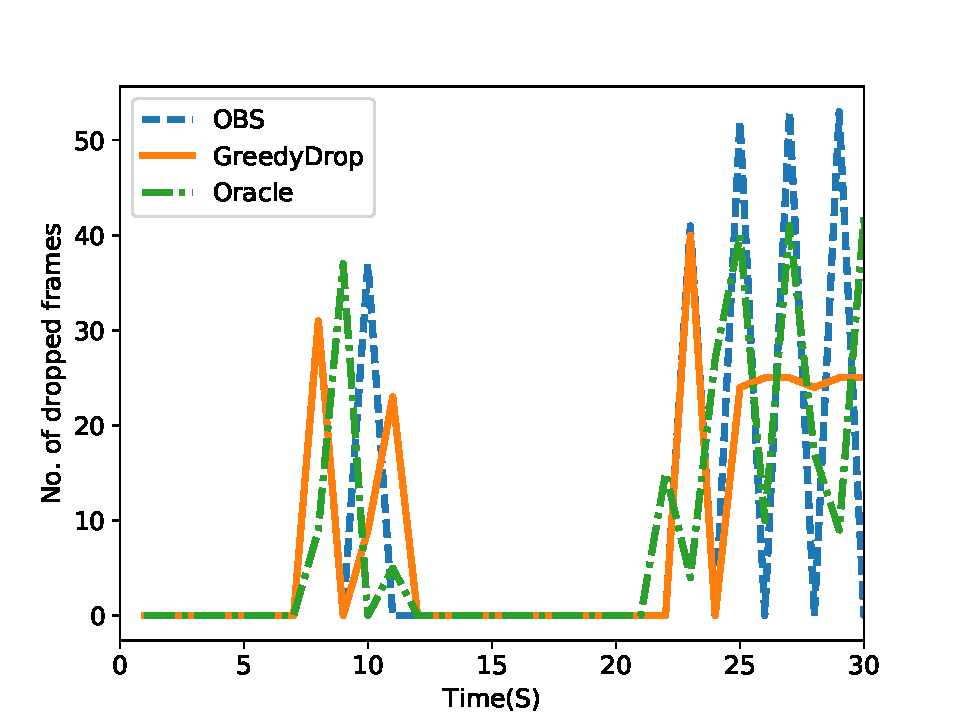
\includegraphics[width=\linewidth]{fig/drop-buffer.pdf}
\caption{No. of frame drop}
\label{fig:drop-buffer}\mylabel{fig:drop-buffer}
\end{subfigure}
\begin{subfigure}[b]{.45\columnwidth}
\centering
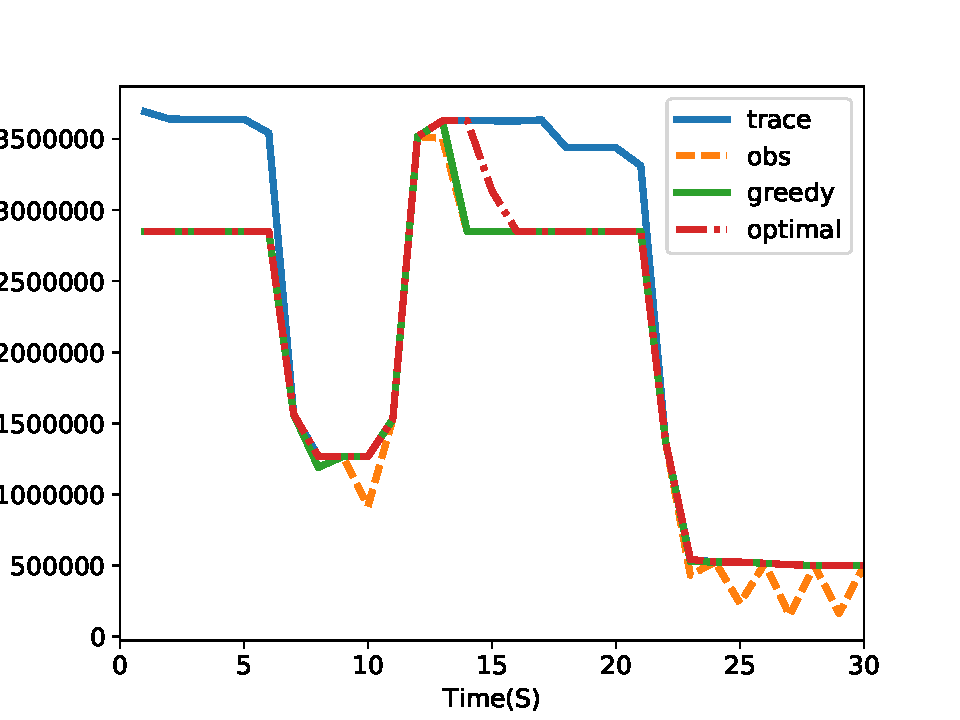
\includegraphics[width=\linewidth]{fig/drop-bandwidth.pdf}
\caption{Real-time throughput}
\label{fig:drop-bandwidth}\mylabel{fig:drop-bandwidth}
\end{subfigure}
\caption{Comparison of different frame drop strategy}
\vspace{-0.15in}
\end{figure} 
The number of dropped frames is displayed in the table ~\ref{tab_drop}. OBS dropped the most frames among three, and greedy reduce $14.4\%$, which is a notable improvement. And the gap between greedy and DP is small, less than $3\%$. The real-time buffer and throughput is showed in Figures ~\ref{fig:drop-buffer}~\ref{fig:drop-bandwidth}, greedy algorithm has the similar behaviour with the obs, but the greedy algorithm achieves a higher minimum number of buffered frames, because greedy only drops the undecodable frames of the first GoP. Thus, the throughput when network recovers of the greedy algorithm is higher than obs. Considering both time complexity and the frame dropping, greedy is the one.

\subsection{Adaptive Bitrate}
\subsubsection{Problem Formulation}
\begin{table}[tb]
\centering
\caption{Terminology in Adaptive Bitrate}
\label{tbl:vbrval}
{\setlength{\tabcolsep}{1pt}
\begin{tabular}{|c|c|l|}
\hline
\textbf{Symbol} & \textbf{Type} & \textbf{Meaning}                      \\ \hline
$j$               & index         & frame index                            \\ \hline
$R_j$             & variable      & the bitrate of frame $j$ \\ \hline
$N_j$             & variable      & No. of the GoPs at time $j$     \\ \hline
$D_j$             & variable      & whether frame $i$ is dropped at time $j$  \\ \hline
$Send_j$             & variable   & No. of frame send at time $j$ \\ \hline
$C_j$              & variable         & network bandwidth at time $j$           \\ \hline
$T_k^j$               & variable         &the remaining time of $k$ GoP at time $j$  \\ \hline
$R_k^j$            & variable         & the bitrate of $k$ GoP at time $j$  \\ \hline
$Drop_j$       & variable & whether the drop would happen at time $j$ \\ \hline
$T$               & const         & decision time                        \\ \hline\end{tabular}}
\end{table}

\begin{eqnarray}
&Max& \sum R_j- \alpha\sum|R_{j+1}-R_j|-\beta\sum D_j
\label{vbr-formulation} \mylabel{vbr-formulation}
\end{eqnarray}
\\ subject to
\begin{eqnarray}
% \nonumber % Remove numbering (before each equation)
&& R_{j+1}=R_j, \forall mod(j,M)\not\equiv M-1 \label{vbr-bitrate}\\
&& S_j = argmax{\sum_k R_k^j*T_k^j \leq C_j}, \forall j \label{vbr-send} \\
&& Rest_j = (C_j- \sum_{S_j} R_k^j*T_k^j)/R_{S_j+1}^j, \forall j \\
&& F_j = sgn(\sum_{S_j+1} T_k^j - Rest_j-T_1), \forall j \label{vbr-drop}\\
&& D_j = F_j*(T_{S_j+1}^j-Rest_j), \forall j \label{vbr-drop-no} \\
&& N_{j+1}=N_j-S_j-F_j+1-sgn(mod(j,M)), \forall j \label{vbr-gop-no}\\
&& R_k^{j+1}=R_{k+S_j+F_j}^j, \forall j, k\in \{1,N_j-S_j-F_j\} \label{vbr-bitrate-next}\\
&& R_{N_j-S_j-F_j+1}^{j+1} = R_{j+1}, \forall mod(j,M) \equiv 0 \label{vbr-bitrate-spec} \\
&& T_k^{j+1} = T_{k+S_j+F_j}^j, \forall j, k\in\{1, N_j-S_j-F_j\} \label{vbr-time-next} \\
&& T_{N_j-S_j-F_j}^{j+1} = T_{N_j-S_j-F_j}^{j+1} - D_j - Rest_j , \forall j \label{vbr-time-spec} \\
&& T_{N_j-S_j-F_j+1}^{j+1}=1, \forall mod(j,M)\equiv 0 \label{vbr-time-spec2} \\
\end{eqnarray}

In this section, we try to handle the long-term bandwidth fading issue. From the distribution of the bandwidth, we use the idea of adaptive bitrate similar with DASH. We use the proposed greedy strategy as the frame dropping strategy. Different from formulation upside, here how to choose the best bitrate is our point. Thus introduce a variable $R_{i}$. $R_{i}$ represents the bitrate of the $i$ frame. Problem can be formulated as follows. Variables is all defined in Table~\ref{tbl:vbrval}. For variable bitrate, calculating how much frames can be send is a tricky problem, because different frames have different size. Constraint $(2)$ requires that bitrate within one GoP must keep the same; $(3)$ calculates the most number of GoPs can be send, constraint $(4)$ judges whether the remaining time after sending exceeds the buffer limit. Equation $(5)$ is the number of dropped frames. Constraints $(6)-(11)$ show the state transition of the bitrate and time of several GoPs.

Offline optimal is hard to calculate. Guess for each GoP, the broadcaster can choose one from total $M$ candidates. For a $T$ GoP decision, the computation complexity equals to $M^T$, a exponential complexity.

\subsubsection{Effective Solution}
\begin{algorithm}[h]
\caption{Greedy Video Adaptation Workflow}
\label{alg:greedy-vbr}\mylabel{alg:greedy-vbr}
\begin{algorithmic}[1]
\State Initialize
\For{j=1 to T}
\State $C_j := ThroughpurPred(C_{[\tau,j-1]})$
\State $R_j := FindClosestBr(C_j)$
\State $D_j := f(C_j, R_j)$
\EndFor
\end{algorithmic}
\end{algorithm} 
\textbf{Algorithm Description.} A exponential complexity issue is hard to calculate in limited time. Besides, the offline optimal is on the basis of given prefect knowledge of future bandwidth. Such long-term bandwidth prediction is inaccurate. A intuitive idea is to change the bitrate following the bandwidth. At time $j$, the broadcaster carries out the following two key steps, as shown in Algorithm ~\ref{alg:greedy-vbr}.

$1.$ Bandwidth estimate. According to Festive and MPC, harmonic mean is a useful method of estimating the future bandwidth. Besides, proposing a prediction mechanism is not the focus.

$2.$ Bitrate choose. Avoid from frequent frame dropping, an appropriate bitrate is essential. Given the future bandwidth $C_j$, an heuristic choice is to choose the highest available bitrate lower than $C_j$.

\textbf{Evaluation.} Buffer-based algorithm preforms excellently in DASH. But in live streaming scenario, the buffer only lasts for $0.7-0.9$ seconds, buffer-based is hard to apply and can only make little difference. But the bitrate-based algorithm still can use. Inspired from ~ref{Xiaoqi Yin}, the state-of-art MPC is used as the baseline.

\begin{figure*}[htb]
\minipage{0.32\textwidth}
  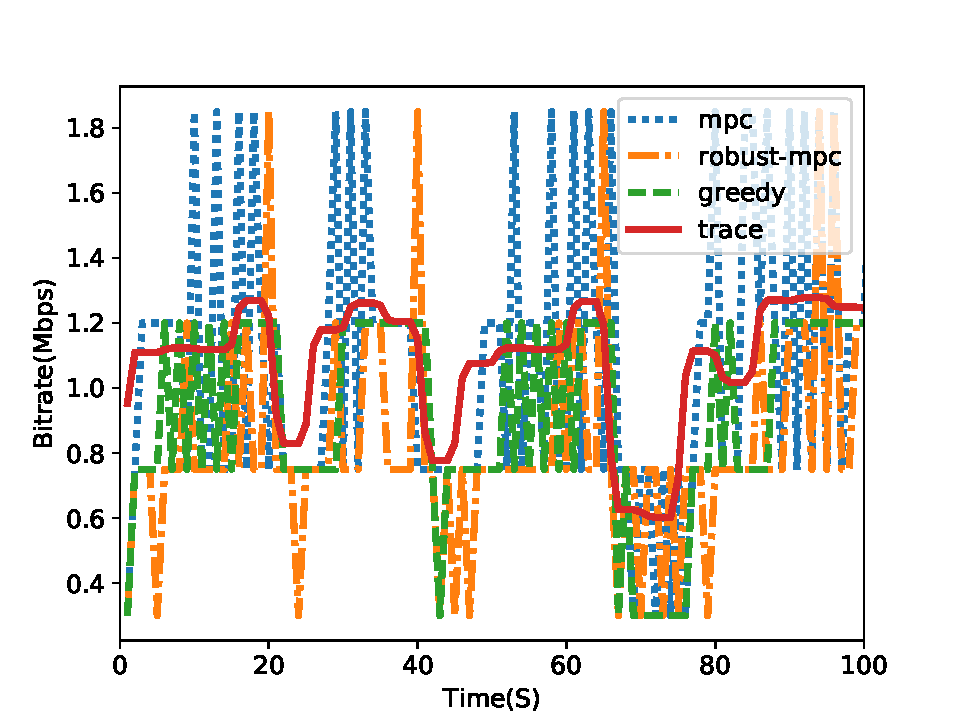
\includegraphics[width=\linewidth]{fig/specific_fcc.pdf}
  \caption{Throughput of FCC dataset}
  \vspace{-0.23in}
  \label{fig:fcc_specific}\mylabel{fig:fcc_specific}
\endminipage
\hfill
\minipage{0.32\textwidth}
  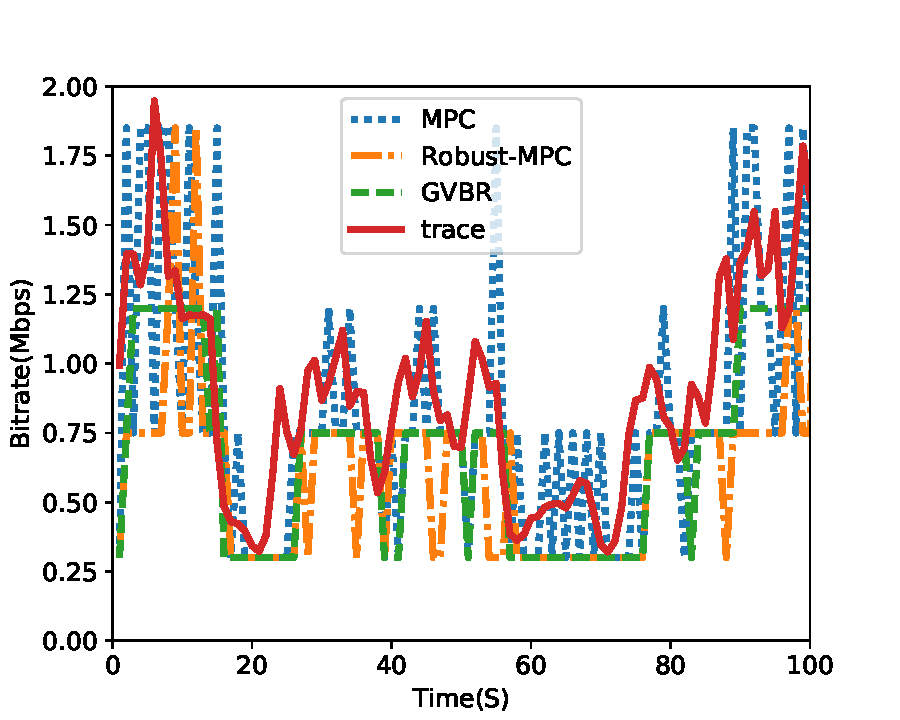
\includegraphics[width=\linewidth]{fig/specific_hsdpa.pdf}
  \caption{Throughput of HSDPA dataset}
  \vspace{-0.23in}
  \label{fig:specific_hsdpa}\mylabel{fig:specific_hsdpa}
\endminipage
\hfill
\minipage{0.32\textwidth}
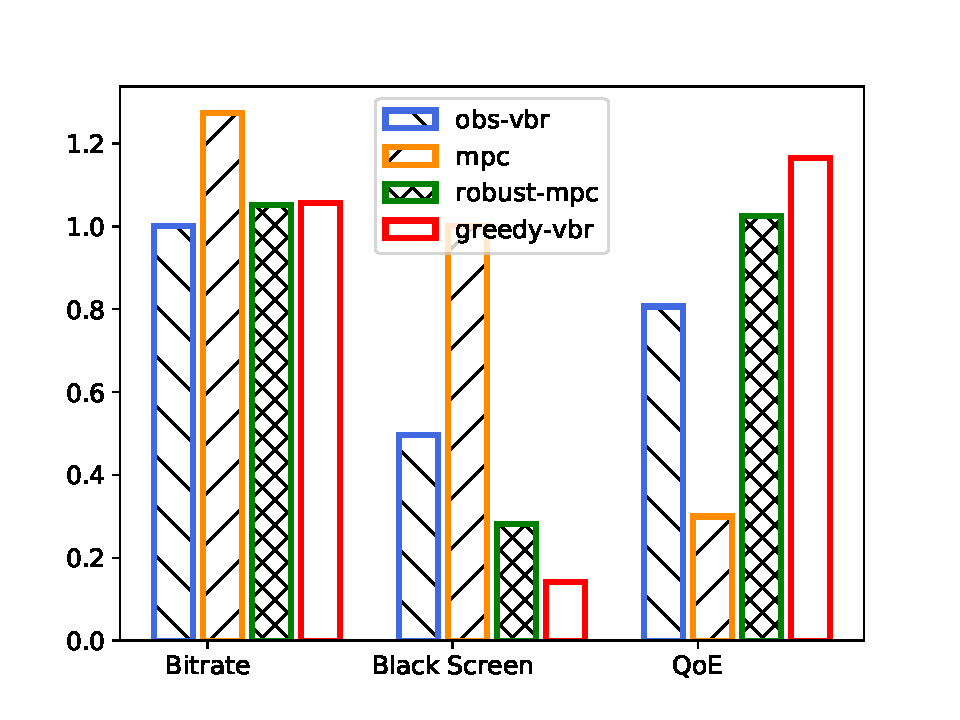
\includegraphics[width=\textwidth]{fig/massive_qoe.pdf}
\caption{Normalized bitrate, play failure and QoE}
\vspace{-0.23in}
\label{fig:vbr-qoe}\mylabel{fig:vbr-qoe}
\endminipage
\end{figure*}

\begin{figure*}[htb]
\minipage{0.32\textwidth}
  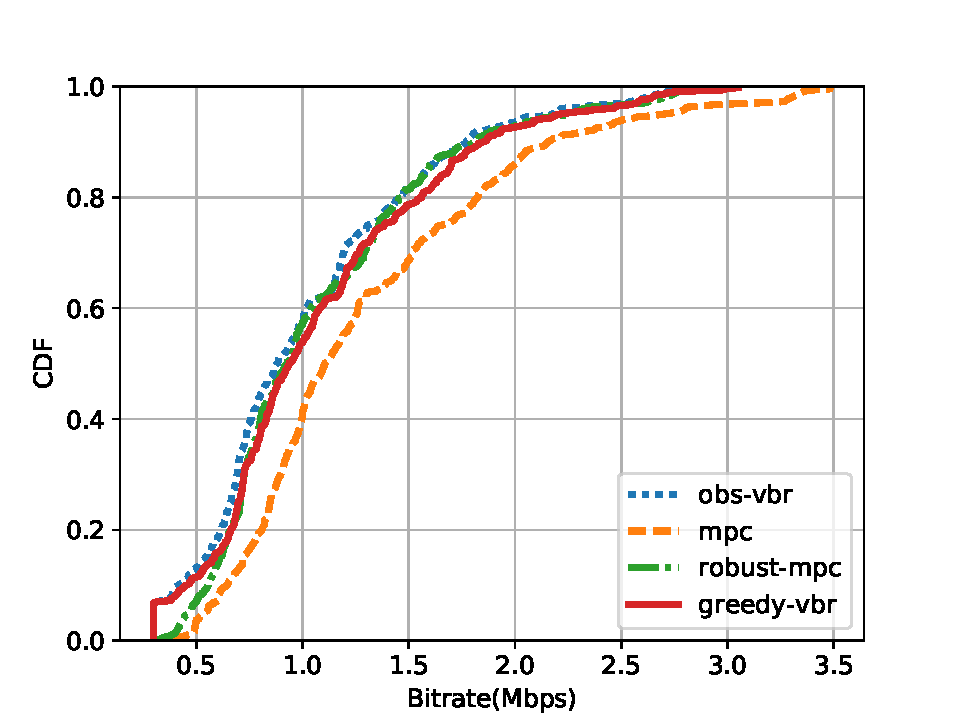
\includegraphics[width=\linewidth]{fig/massive-bitrate-cdf.pdf}
  \caption{CDF of Bitrate}
  \vspace{-0.25in}
  \label{fig:vbr-bitrate-cdf}\mylabel{fig:vbr-bitrate-cdf}
\endminipage
\minipage{0.32\textwidth}
  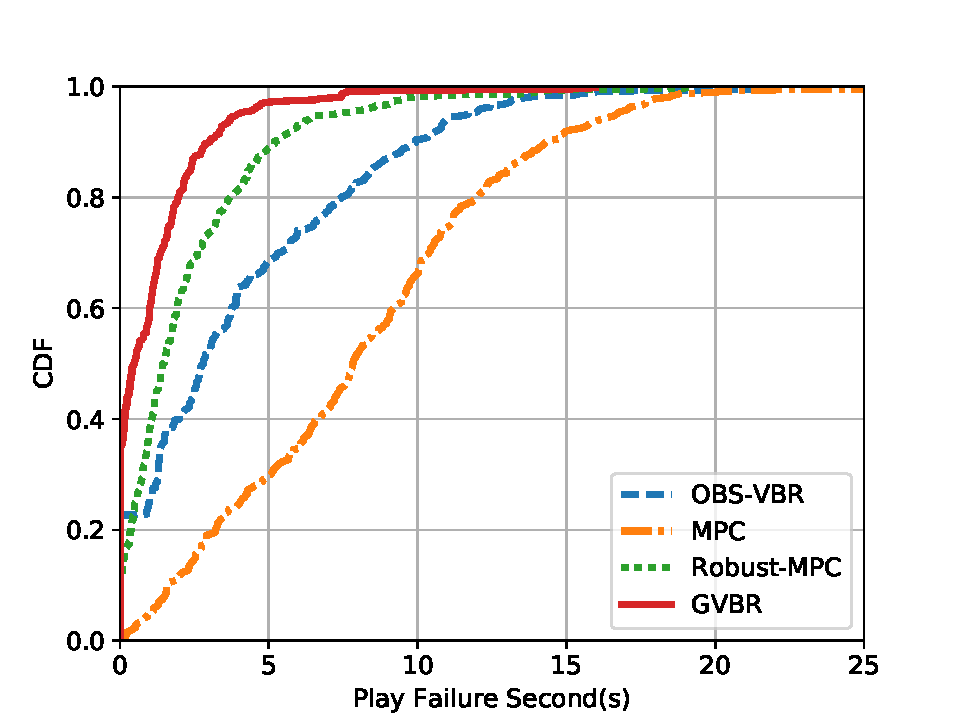
\includegraphics[width=\linewidth]{fig/massive-drop-cdf.pdf}
  \caption{CDF of Play Failure Seconds}
  \vspace{-0.25in}
  \label{fig:vbr-drop-cdf}\mylabel{fig:vbr-drop-cdf}
\endminipage
\minipage{0.32\textwidth}
  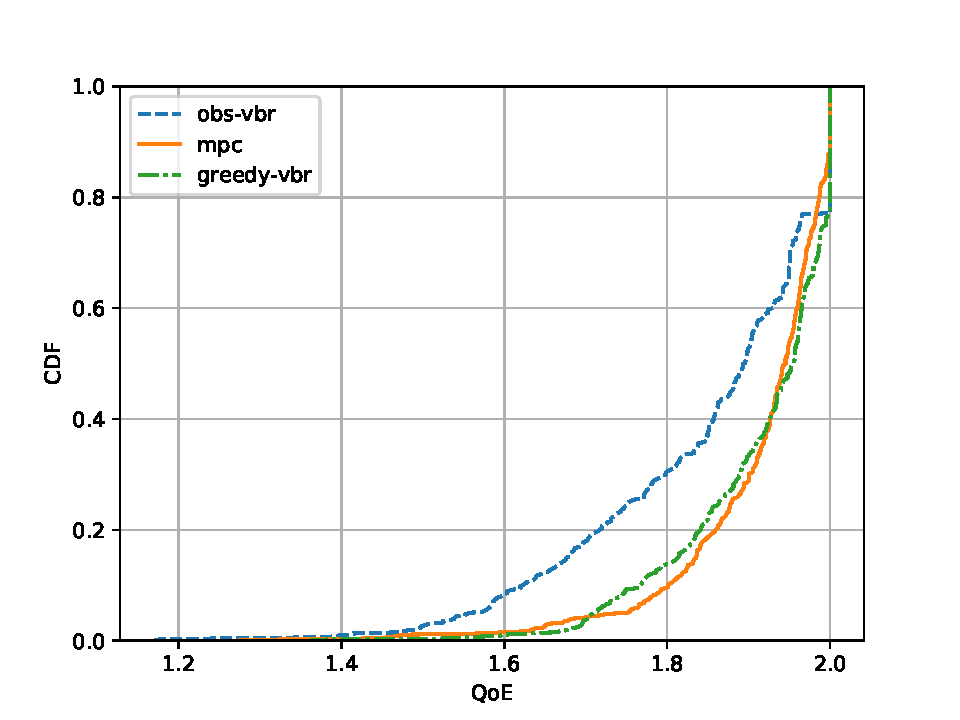
\includegraphics[width=\linewidth]{fig/massive-qoe-cdf.pdf}
  \caption{CDF of Normalized QoE }
  \vspace{-0.25in}
  \label{fig:vbr-qoe-cdf}\mylabel{fig:vbr-qoe-cdf}
\endminipage
\end{figure*} 
We compared four algorithm together. First is the obs default algorithm, constant bitrate, and the default drop strategy. Second, change the constant bitrate into the greedy algorithm. Third, compare the greedy drop strategy plus the RHC. And the last one, our own greedy bitrate chosen algorithm plus the greedy drop strategy. Specific comparison results are shown in Figures ~\ref{fig:vbr-qoe}.

These algorithms reach almost the same average bitrate, with little difference. Because for all of these algorithms, the real-time bitrate waves around the average bandwidth. The first CBR algorithm drops the most frames, more than 5 times when compared with other VBR algorithms. Introducing the idea of VBR reduces the dropped frames to a acceptable level, at most $5$ seconds. QoE equals to the weighted sum of three key factors. In our case, frame dropping takes the most important roles, the value of QoE almost follows the frame dropping. MPC and our proposed greedy algorithm perform almost the same in QoE and frame dropping. Default OBS always has a poorer qoe than other three algorithms. The following cdf shows the specific distribution of all the three indexes, similar with the average pictures.
